\chapter{Selection of Dynamical Reputation Model parameters}
\label{App:parameters}

The Dynamical Reputation Model(DIBRM) has several tuning parameters. In previous studies, the model \cite{melnikov2018toward,yashkina2020} was used to approximate real reputation on Stack Exchange sites \cite{yashkina2020}, so model parameters were $t_a =2, \beta = 1, \alpha = 1.4$, while the basic reputation value $I_{bn}$ was +2 or +4. As $\beta=1$, the forgetting factor is not considered. Our goal was to describe how reputation influences the sustainability of the community. Further, we wanted to resemble the concept of trust. Our tuning procedure differs from previous studies on Stack Exchange sites, and we ended up with different model parameters. 

For \textbf{basic reputation contribution}, we selected $I_{bn}=1$. With these values, each interaction has an initial contribution $+1$. 

For \textbf{characteristic time} $t_a$ we choose $t_a=1$. The median/average time between subsequent interactions is $1 day$. If the time window between two interactions is less than $1 day$, their reputation will rise; otherwise, the reputation decays.

\begin{figure}[h]
	\centering
	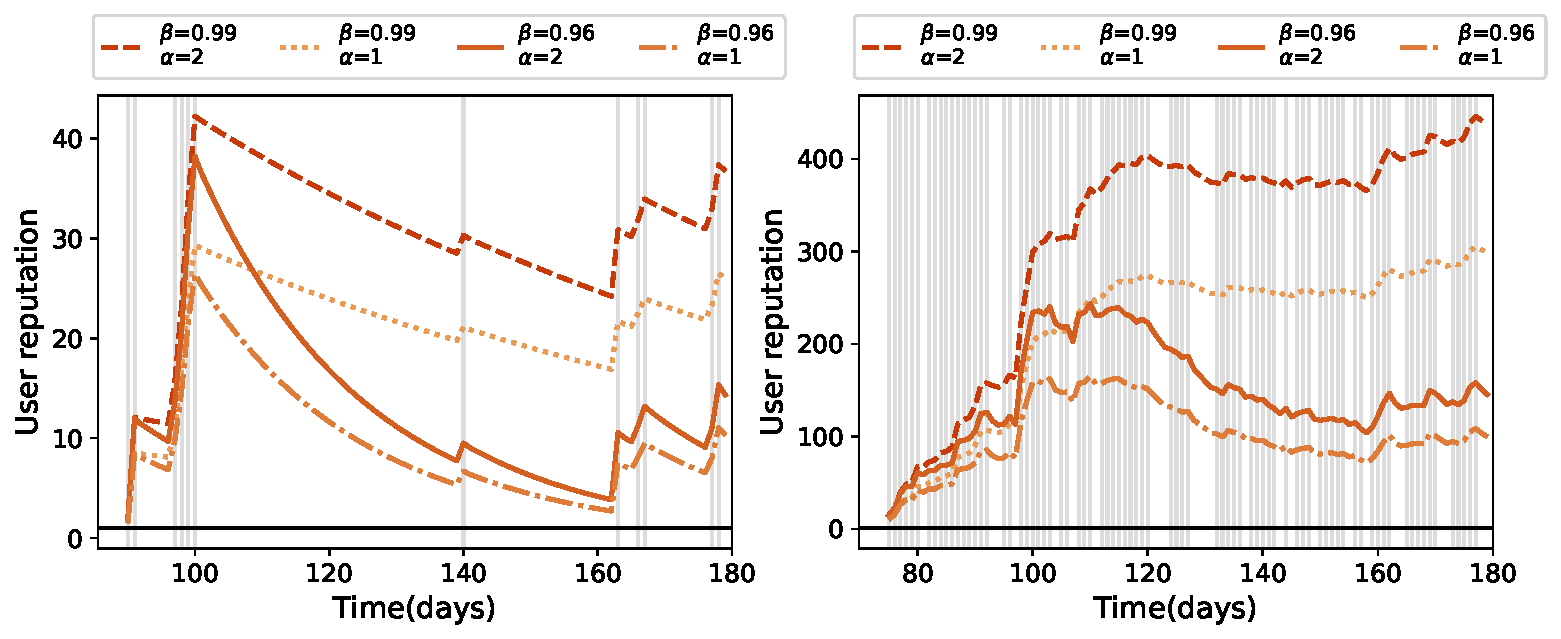
\includegraphics[width=0.8\linewidth]{figures/stackexchange/single_user_reputation.pdf}
	\caption[Single users reputations.]{Single users reputations }
	\label{fig:singleuser}
\end{figure} 

The {parameter $\alpha$} represents the \textbf{cumulative factor}. The burst in activity and recent interactions lead to higher reputation values with larger parameter $\alpha$. Figure \ref{fig:singleuser} represents the reputations of two selected users from SE. The first is sporadically active, while the second makes frequent interactions. We calculate the reputation of these two users for different parameters $(\alpha, \beta)$. We selected $\alpha=2$.  

The reputation decay determines the \textbf{forgetting factor $\beta$}. We set the parameter on $\beta=0.96$. The reputation should reflect the properties of the trust. This means we do not expect $\beta$ to be high, as inactive users keep larger reputation values. In Figure \ref{fig:singleuser} for $\beta=0.99$, even for the little active user, reputation stays higher during the observed period. With lower $\beta$, it may drop to the reputation threshold and indicate that the user stopped to be active.  

We compared the number of users with an estimated reputation higher than 1 for different parameters $\beta$. We concluded that $\beta$ close to $0.96$ approximates the number of users with recorded interactions in a given 30-day sliding window. For each pair of communities, we calculated the number of users with at least one interaction in every 30-day sliding window. Then we estimated several times in series expressing the number of users with a reputation higher than 1 for fixed $\beta$. Then we calculated the root mean square error (RMSE) between those time series for the first 200 days. Values of RMSE are shown in Figure~\ref{fig:rmse}. For each community, we can find parameter $\beta$ that minimizes RMSE. Although $\beta$ does not have a unique value across communities, it varies between 0.95 and 0.96.  

\begin{figure}[h!]
	\centering
	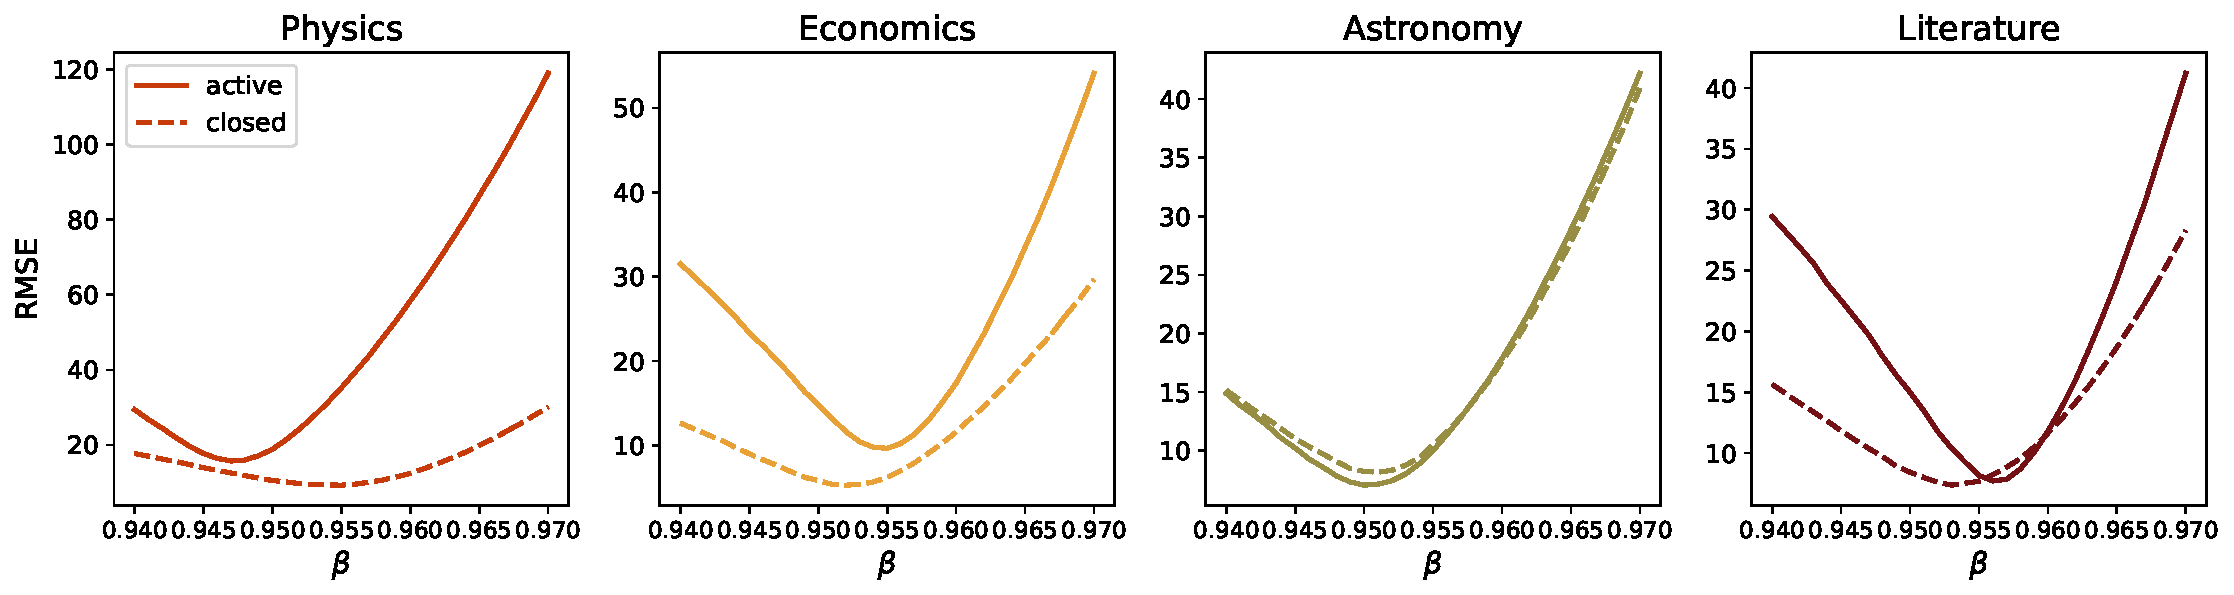
\includegraphics[width=\linewidth]{figures/stackexchange/rmse.pdf}
	\caption[RMSE between the number of users in 30 days sliding window and positive reputation.]{RMSE between the number of active users in a sliding window of 30 days and the number of users with reputation $>1$ for  $0.94< \beta <0.97$ with step $0.001$. }
	\label{fig:rmse}
\end{figure}

Figure \ref{fig:nusers} compares the number of users in the 30-day sliding window and the number of users for these optimal values $\beta = 0.954$ and $\beta =0.96$. For $\beta = 0.96$, we observe that the estimated number of active users in most communities is consistently slightly higher than the actual number of users who have made at least one interaction in that sliding window. This means that the dynamic reputation model sometimes overestimates the user's reputation, but it is far more important because it never underestimates the real number of active users. Since we base our calculations of total and average reputation within the community only on users whose reputation is higher than the threshold, this is important as the model disregards no active users due to the value of the decay parameter.

\begin{figure}[H]
	\centering
	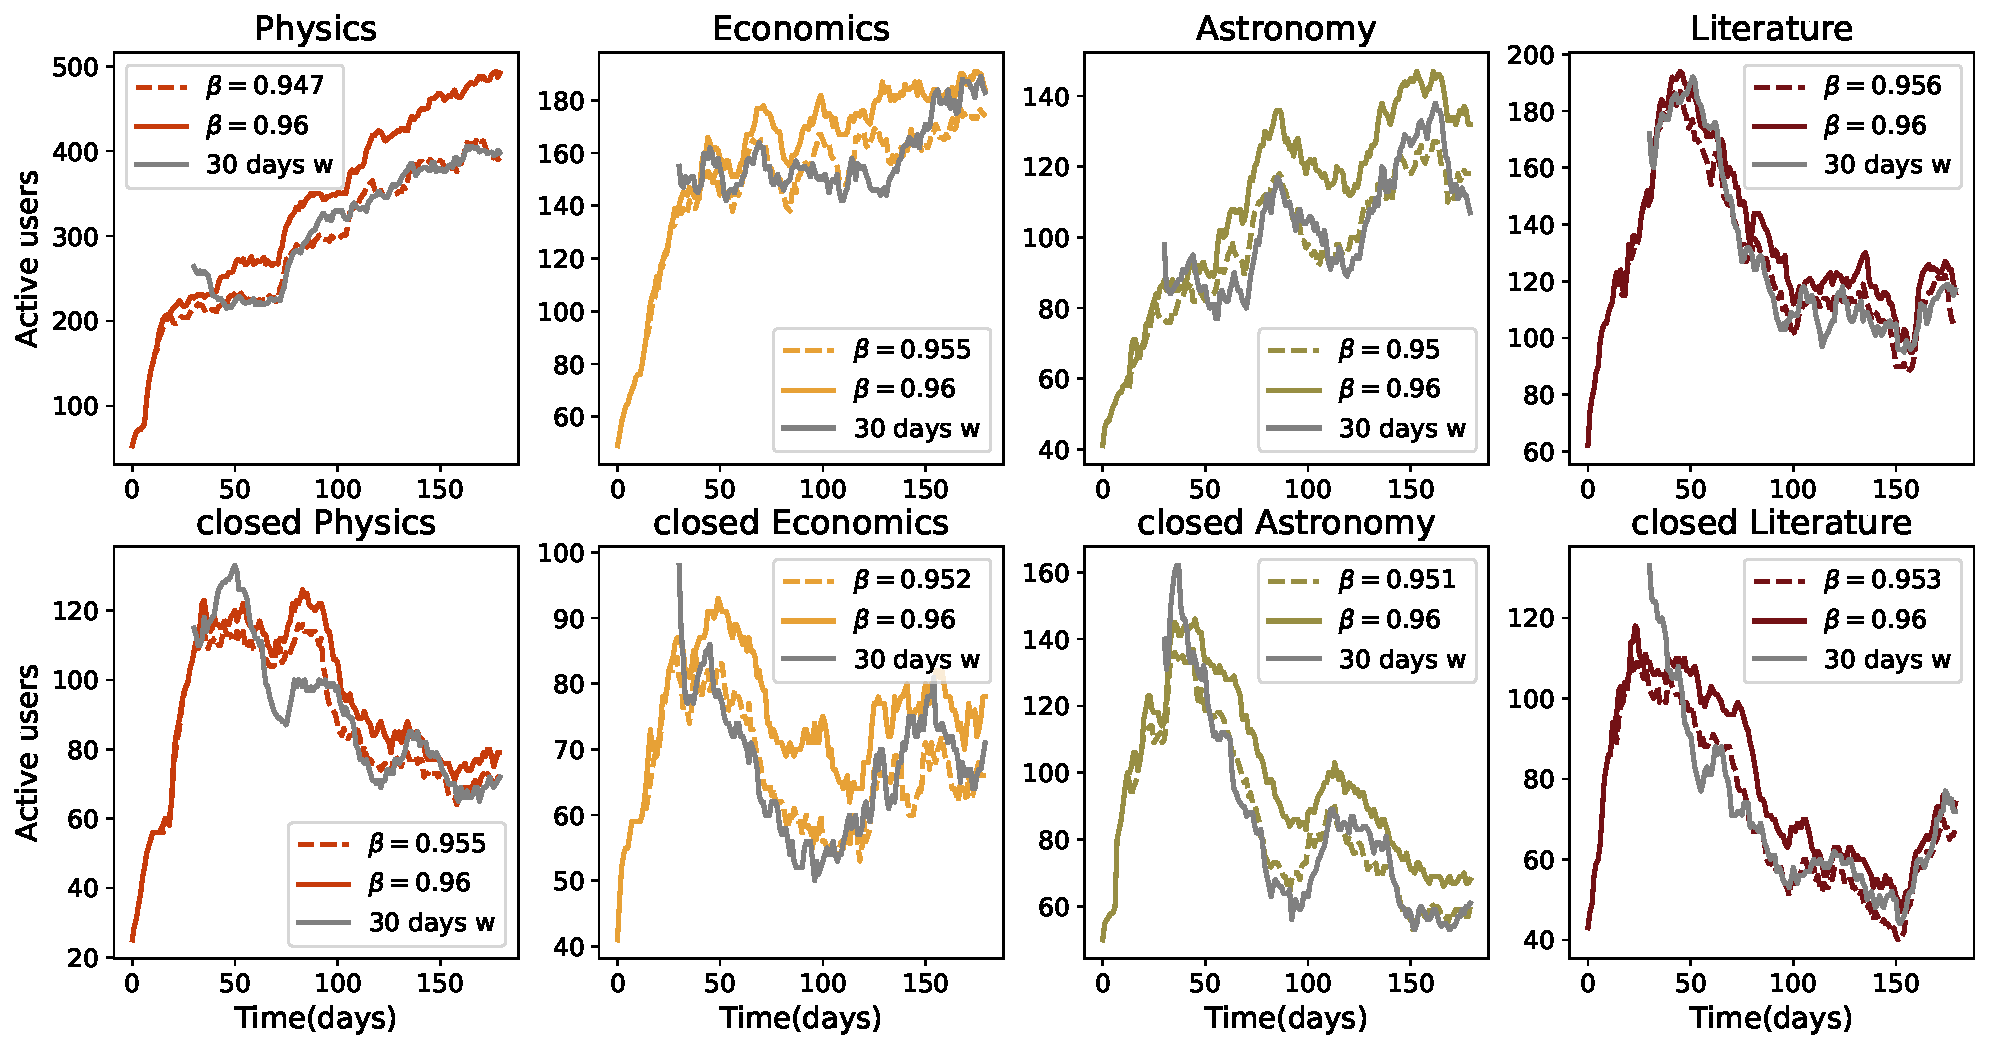
\includegraphics[width=\linewidth]{figures/stackexchange/active_users.pdf}
	\caption[Number of users in 30 days sliding window and positive reputation.]{Number of active users in a sliding window of 30 days and number of users with dynamic reputation higher than 1 for $\beta=0.954$ and $\beta=0.96 $ which provide the best fit to the number of users in 30 days sub-networks for each community}
	\label{fig:nusers}
\end{figure}

Finally, it's important that our dynamic reputation captures the trend of long-term user activity. In Figure~\ref{fig:active-users}, solid lines show the time series of an estimated dynamic reputation for $\beta = 0.96$ while dashed lines show the number of active users in a given sliding window and continued to be active in the next one. Although the total estimated number of active users is expectedly to be higher, the two-time series follows similar trends in different communities.

\begin{figure}[H]
	\centering
	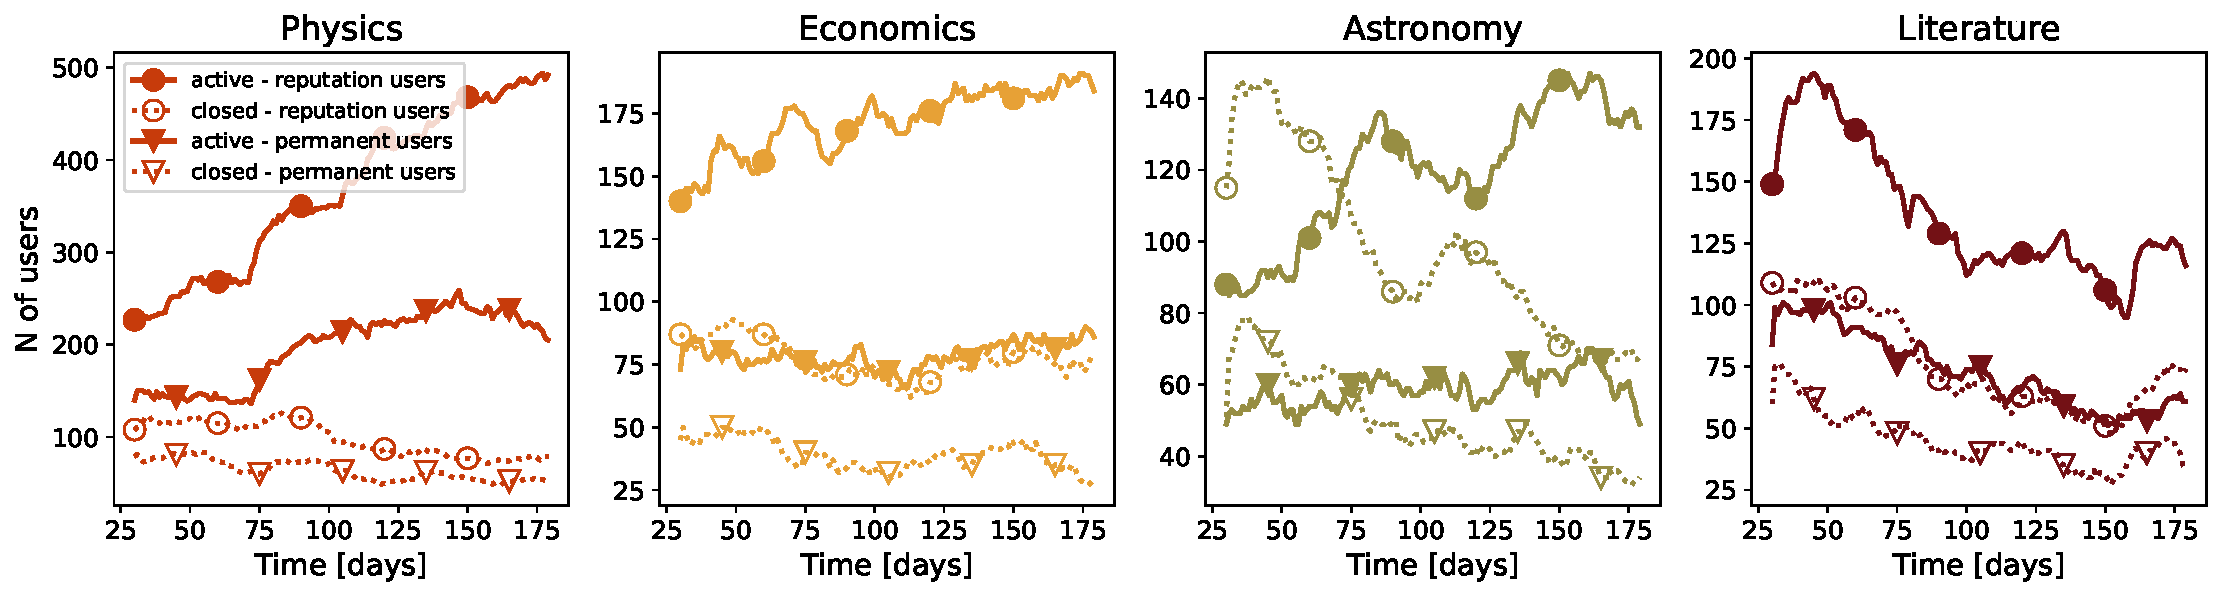
\includegraphics[width=1\linewidth]{figures/stackexchange/permanent_users.pdf}
	\caption[Number of users in Stack Exchange community who remain to be active]{Solid lines represent the number of users with dynamic reputation higher than 1 for $\beta=0.96$ while dashed lines are the number of users within 30 days sliding window who were active and remained to be active. Blue lines are beta, while red lines are area51 communities.}
	\label{fig:active-users}
\end{figure}

\clearpage
